\documentclass[11pt, a4paper]{article}
\usepackage[utf8]{inputenc}
\usepackage[spanish]{babel}
\usepackage{amsmath, amssymb, amsfonts}
\usepackage{graphicx}
\usepackage{geometry}
\geometry{left=2.5cm, right=2.5cm, top=2.5cm, bottom=2.5cm}
\usepackage{tikz}
\usepackage{bm}
\usepackage[hidelinks]{hyperref}
\graphicspath{{figs/}{../figs/}}


\title{\vspace{-1.5cm}\textbf{Resolución de Ecuaciones Diferenciales Ordinarias}\\ \large Métodos Matemáticos I --- Hoja 3}
\author{\textbf{César Endris Acosta}}

\date{8 de octubre de 2026}
\begin{document}

\maketitle
\vspace{-0.2cm}

\begin{center}
\fbox{\parbox{0.93\linewidth}{\small
\textbf{Versión interactiva.} Todos los problemas de esta hoja se pueden visualizar e interactuar con sus gráficas
(constantes con deslizadores, curva elegida, campos de direcciones, etc.) en la página web
(pestaña ``Hoja 3''):\\[2pt]
\centerline{\url{https://endris10.github.io/Mathematical_Methods_1/}}\vspace{2pt}
Se utilizó IA (Claude, de Anthropic) \textbf{únicamente para programar la página web};
la resolución de las ecuaciones diferenciales es propia.}}
\end{center}

\noindent\textbf{1. Integrad la EDO: $\bm{(x^4\ln x - 2xy^3)dx + 3x^2y^2dy = 0}$} \\
$M(x,y) = x^4\ln x - 2xy^3$ y $N(x,y) = 3x^2y^2$:
\begin{align*}
\frac{\partial M}{\partial y} = -6xy^2, \qquad \frac{\partial N}{\partial x} = 6xy^2 \implies \text{No es exacta.}
\end{align*}
\begin{align*}
\frac{\partial}{\partial y}\big(M(x,y)\mu(x)\big) = \frac{\partial}{\partial x}\big(N(x,y)\mu(x)\big)
\end{align*}
\begin{align*}
\mu(x)\frac{\partial M}{\partial y} &= \mu'(x)N(x,y) + \mu(x)\frac{\partial N}{\partial x}
\end{align*}
\begin{align*}
\mu(x)(-6xy^2) &= \mu'(x)(3x^2y^2) + \mu(x)(6xy^2)
\end{align*}
\begin{align*}
\mu'(x) &= \frac{-12xy^2}{3x^2y^2} \, \mu(x) \implies \mu'(x) = -\frac{4}{x} \, \mu(x)\implies \mu(x) = e^{\int -\frac{4}{x}dx} = \frac{1}{x^4}
\end{align*}

Comprobamos la exactitud de la nueva EDO:
\begin{align*}
\frac{\partial}{\partial y}\big(M(x,y)\mu(x)\big) &= \frac{\partial}{\partial y}\left(\ln x - \frac{2y^3}{x^3}\right) = -\frac{6y^2}{x^3} \\
\frac{\partial}{\partial x}\big(N(x,y)\mu(x)\big) &= \frac{\partial}{\partial x}\left(\frac{3y^2}{x^2}\right) = -\frac{6y^2}{x^3}
\end{align*}
Integrando $\tilde{N} = \frac{3y^2}{x^2}$ respecto de $y$ obtenemos $f(x,y) = \frac{y^3}{x^2} + h(x)$. Derivando e igualando a $\tilde{M}$:
\begin{align*}
\frac{\partial f}{\partial x} = -\frac{2y^3}{x^3} + h'(x) = \ln x - \frac{2y^3}{x^3} \implies h'(x) = \ln x \implies h(x) = x(\ln x - 1)
\end{align*}
\[
\boxed{\frac{y^3}{x^2} + x\ln x - x = C}
\]


\begin{center}
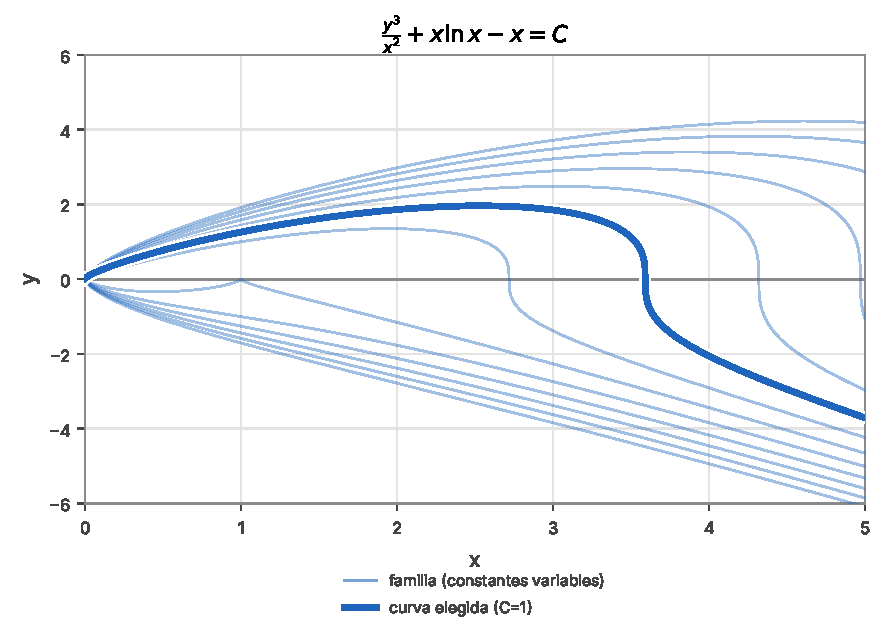
\includegraphics[width=0.8\linewidth]{h3-01.pdf}
\end{center}

\noindent\textbf{2. Integrad la EDO: $\bm{(x+\sin x+\sin y)dx + \cos y \, dy = 0}$} \\
$M(x,y) = x+\sin x+\sin y$ y $N(x,y) = \cos y$:
\begin{align*}
\frac{\partial M}{\partial y} = \cos y, \qquad \frac{\partial N}{\partial x} = 0 \implies \text{No es exacta.}
\end{align*}
\begin{align*}
\frac{\partial}{\partial y}\big(M(x,y)\mu(x)\big) = \frac{\partial}{\partial x}\big(N(x,y)\mu(x)\big)
\end{align*}
\begin{align*}
\mu(x)\cos y &= \mu'(x)\cos y + \mu(x)(0)
\end{align*}
\begin{align*}
\mu'(x) = \mu(x) \implies \mu(x) = e^x
\end{align*}

Comprobamos la exactitud de la nueva EDO:
\begin{align*}
\left.\begin{aligned}
\frac{\partial \tilde{M}}{\partial y} &= \frac{\partial}{\partial y}\big(e^x(x+\sin x+\sin y)\big) = e^x\cos y \\[1.5ex]
\frac{\partial \tilde{N}}{\partial x} &= \frac{\partial}{\partial x}(e^x\cos y) = e^x\cos y
\end{aligned}\right\} \implies \text{Oh sorpresa, es exacta.}
\end{align*}
Integrando $\tilde{N} = e^x\cos y$ respecto de $y$ tenemos $f(x,y) = e^x\sin y + h(x)$. Derivando e igualando a $\tilde{M}$:
\begin{align*}
\frac{\partial f}{\partial x} = e^x\sin y + h'(x) = e^x(x+\sin x+\sin y) \implies h'(x) = e^x(x+\sin x)
\end{align*}
Integrando $h'(x)$ por partes:
\begin{align*}
h(x) = \int e^x(x+\sin x) dx = e^x(x-1) + \frac{e^x(\sin x - \cos x)}{2}
\end{align*}
\[
\boxed{\sin y + x - 1 + \frac{\sin x - \cos x}{2} = C e^{-x}}
\]



\begin{center}
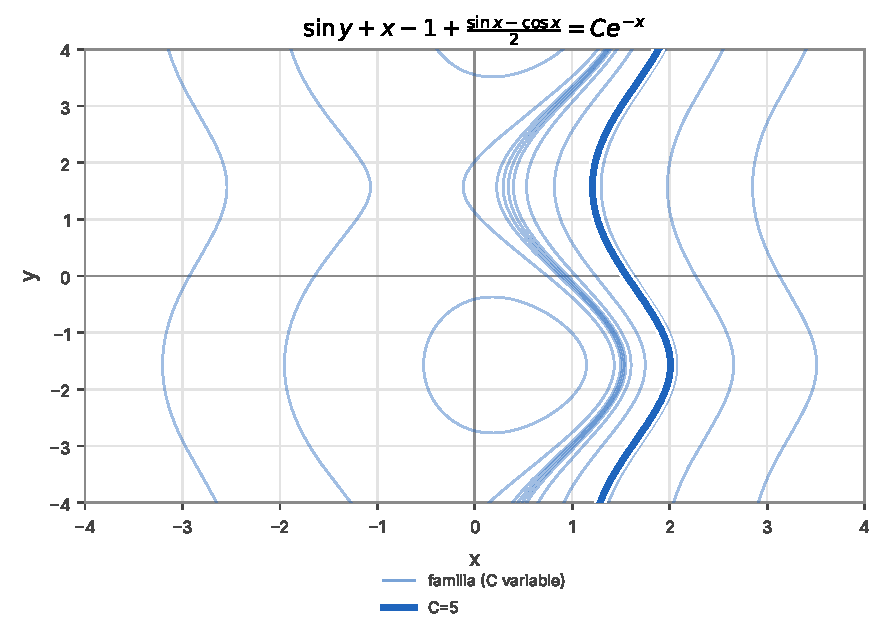
\includegraphics[width=0.8\linewidth]{h3-02.pdf}
\end{center}

\noindent\textbf{3. Integrad la EDO: $\bm{y = (y')^2 e^{y'}}$} \\
$y' = p \implies y = p^2 e^p$. Diferenciando $y$:
\begin{align*}
\frac{dy}{dp} &= (2pe^p + p^2 e^p)dp = p(p+2)e^p
\end{align*}
Como $dy = p dx$, ($p\neq 0$):
\begin{align*}
p dx &= p(p+2)e^p dp \implies dx = (p+2)e^p dp \\
x &= \int (p+2)e^p dp = (p+1)e^p + C
\end{align*}
\textit{Para $p=0$ se obtiene la solución $y=0$ (recuperada en el límite).}
\[
\boxed{\begin{cases} x = (p+1)e^p + C \\ y = p^2 e^p \end{cases}}
\]



\begin{center}
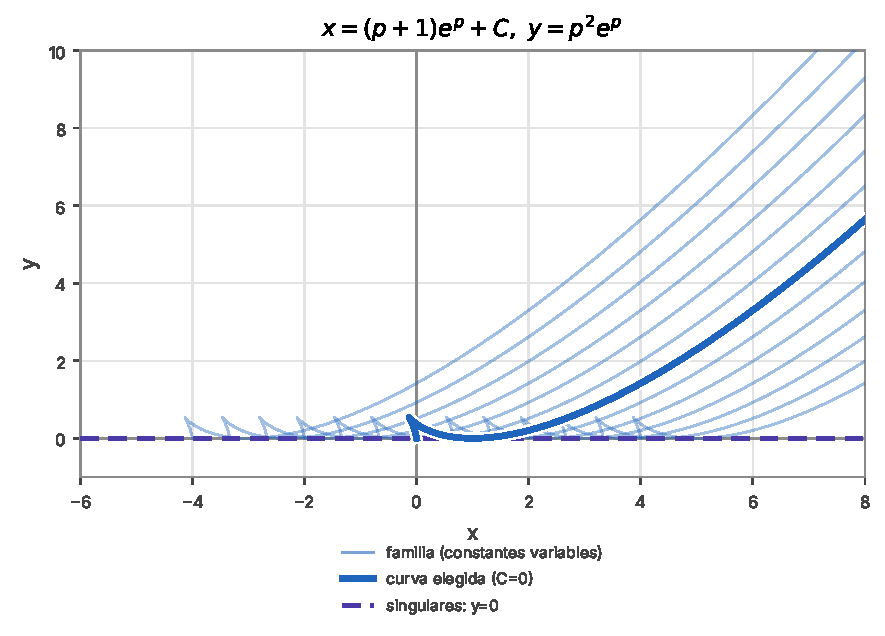
\includegraphics[width=0.8\linewidth]{h3-03.pdf}
\end{center}

\noindent\textbf{4. Integrad la EDO: $\bm{x = \ln y' + \sin y'}$} \\
$y' = p \implies x = \ln p + \sin p$
\begin{align*}
dx &= \left(\frac{1}{p} + \cos p\right)dp
\end{align*}
haciendo $dy = p dx$:
\begin{align*}
dy &= p\left(\frac{1}{p} + \cos p\right)dp = (1 + p\cos p)dp \\
y &= \int (1 + p\cos p)dp = p + p\sin p + \cos p + C
\end{align*}
\[
\boxed{\begin{cases} x = \ln p + \sin p \\ y = p + p\sin p + \cos p + C \end{cases}}
\]



\begin{center}
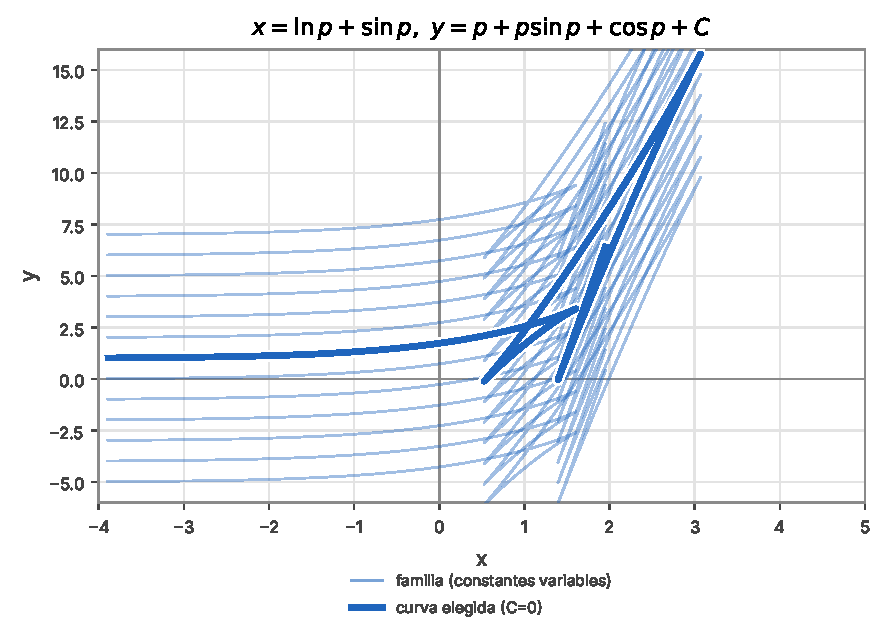
\includegraphics[width=0.8\linewidth]{h3-04.pdf}
\end{center}

\noindent\textbf{5. Integrad la EDO: $\bm{x(1+(y')^2)^{3/2} = a}$} \\
$y' = p \implies x = \dfrac{a}{(1+p^2)^{3/2}}$. Diferenciando $x$:
\begin{align*}
dx &= -\frac{3ap}{(1+p^2)^{5/2}}dp
\end{align*}
Como $dy = p dx$:
\begin{align*}
dy &= -\frac{3ap^2}{(1+p^2)^{5/2}}dp \implies y = -3a\int \frac{p^2}{(1+p^2)^{5/2}}dp
\end{align*}
$p = \tan\theta \implies dp = \sec^2\theta \, d\theta$, con lo que $x = a\cos^3\theta$

\begin{align*}
y &= -3a\int \sin^2\theta\cos\theta \, d\theta = C - a\sin^3\theta
\end{align*}
\[
\boxed{\begin{cases} x = a\cos^3\theta \\[1ex] y = C - a\sin^3\theta \end{cases}}
\]


\begin{center}
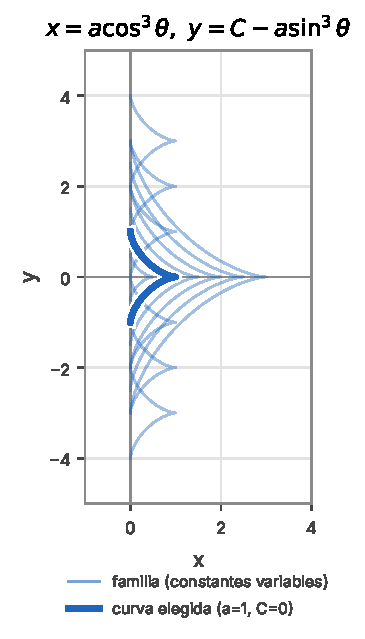
\includegraphics[width=0.8\linewidth]{h3-05.pdf}
\end{center}

\noindent\textbf{6. Integrad la EDO: $\bm{x = y' + \sin y'}$} \\
$y' = p \implies x = p + \sin p$.
\begin{align*}
dx &= (1 + \cos p)dp \quad\quad dy = p dx
\end{align*}

\begin{align*}
dy &= p(1 + \cos p)dp = (p + p\cos p)dp \\
y &= \int (p + p\cos p)dp = \frac{p^2}{2} + p\sin p + \cos p + C
\end{align*}
\[
\boxed{\begin{cases} x = p + \sin p \\ y = \dfrac{p^2}{2} + p\sin p + \cos p + C \end{cases}}
\]



\begin{center}
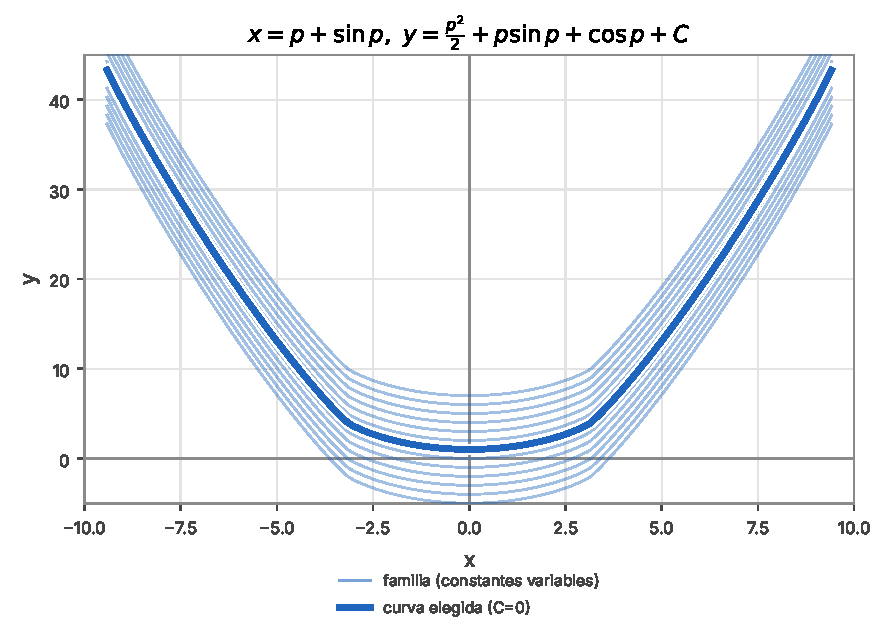
\includegraphics[width=0.8\linewidth]{h3-06.pdf}
\end{center}

\noindent\textbf{7. Integrad la EDO: $\bm{y = 2xy' + \ln y'}$} \\
$y' = p \implies y = 2xp + \ln p$.
\begin{align*}
dy &= 2p dx + 2xdp + \frac{1}{p}dp
\end{align*}
Sustituyendo $dy = pdx$:
\begin{align*}
p dx &= 2p dx + \left(2x + \frac{1}{p}\right)dp \implies \frac{dx}{dp} + \frac{2}{p}x = -\frac{1}{p^2}
\end{align*}
\textit{$x_h = \dfrac{K}{p^2}$ y variando la constante $x(p) = \dfrac{C-p}{p^2}$. Sustituyendo en la expresión de $y(p)$:}
\[
\boxed{\begin{cases} x = \dfrac{C-p}{p^2} \\[2ex] y = \dfrac{2(C-p)}{p} + \ln p \end{cases}}
\]



\begin{center}
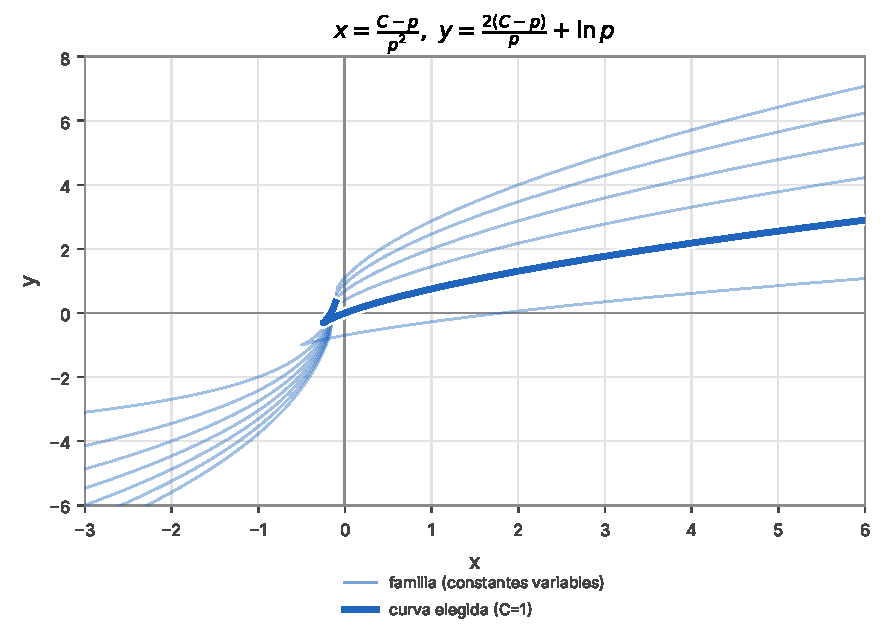
\includegraphics[width=0.8\linewidth]{h3-07.pdf}
\end{center}

\noindent\textbf{8. Integrad la EDO: $\bm{y = 2xy' + \sin y'}$} \\
$y' = p \implies y = 2xp + \sin p$.
\begin{align*}
dy &= 2p dx + 2xdp + \cos p \, dp \qquad dy = pdx 
\end{align*}
\begin{align*}
p dx &= 2p dx + (2x + \cos p)dp \implies \frac{dx}{dp} + \frac{2}{p}x = -\frac{\cos p}{p}
\end{align*}
\textit{Resolvemos la lineal, $x_h = \dfrac{K(p)}{p^2}$ y $x(p) = \dfrac{C - p\sin p - \cos p}{p^2}$.}
\[
\boxed{\begin{cases} x = \dfrac{C - p\sin p - \cos p}{p^2} \\[2ex] y = \dfrac{2(C - \cos p)}{p} - \sin p \end{cases}}
\]



\begin{center}
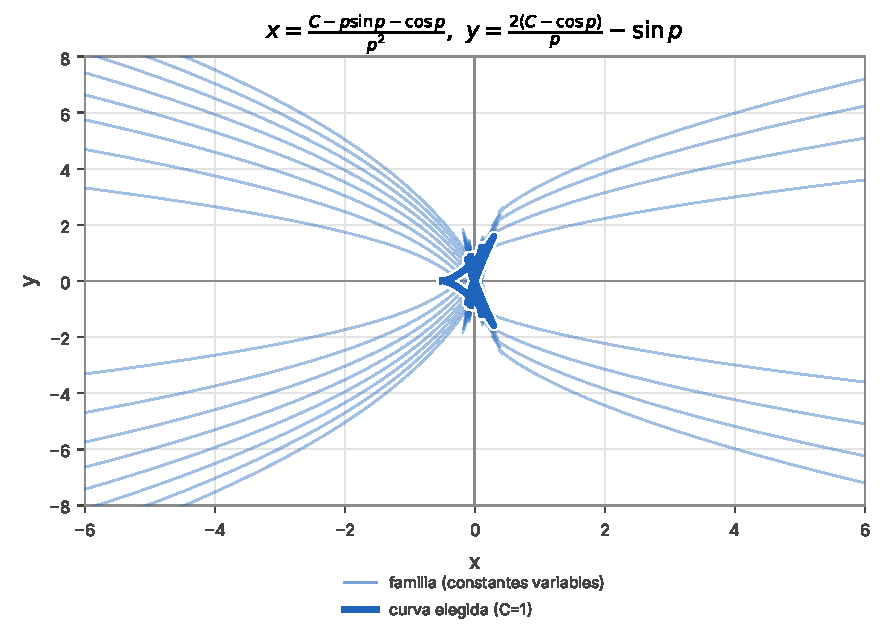
\includegraphics[width=0.8\linewidth]{h3-08.pdf}
\end{center}

\noindent\textbf{9. Integrad la EDO: $\bm{y = x(y')^2 - \frac{1}{y'}}$} \\
$y' = p \implies y = xp^2 - \frac{1}{p}$.
\begin{align*}
dy &= p^2 dx + 2xp \, dp + \frac{1}{p^2}dp \qquad dy=pdx
\end{align*}
\begin{align*}
p dx &= p^2 dx + \left(2xp + \frac{1}{p^2}\right)dp \implies \frac{dx}{dp} - \frac{2}{1-p}x = \frac{1}{p^3(1-p)}
\end{align*}
\textit{Resolviendo la lineal, $x(p) = \dfrac{2Cp^2 + 2p - 1}{2p^2(1-p)^2}$. Además, $p=1 \implies y = x-1$ constituye una solución singular.}
\[
\boxed{\begin{cases} x = \dfrac{2Cp^2 + 2p - 1}{2p^2(1-p)^2} \\[2ex] y = \dfrac{2Cp^2 + 2p - 1}{2(1-p)^2} - \dfrac{1}{p} \end{cases}}
\]



\begin{center}
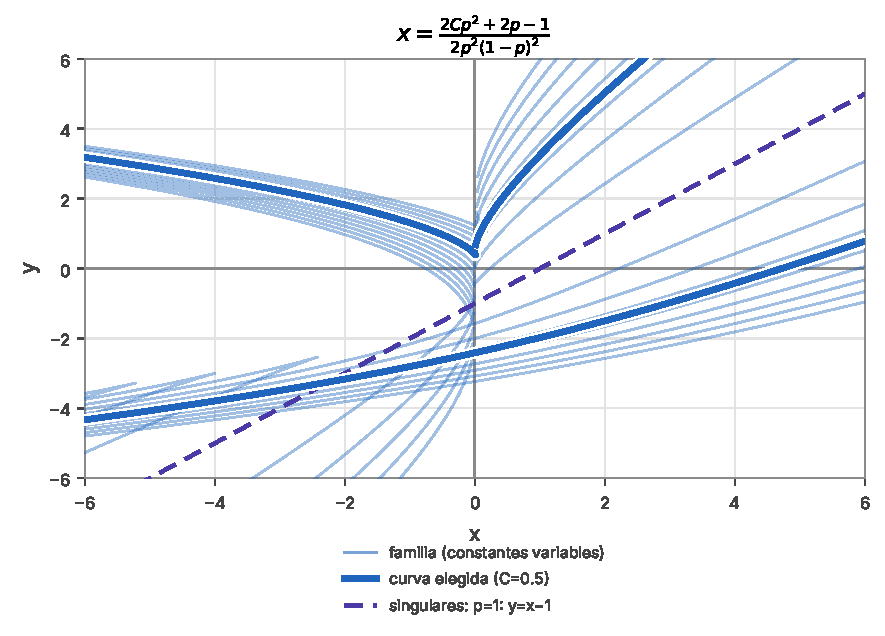
\includegraphics[width=0.8\linewidth]{h3-09.pdf}
\end{center}

\noindent\textbf{10. Integrad la EDO: $\bm{y = xy' + \frac{a}{(y')^2}}$} \\
$y' = p \implies y = xp + \frac{a}{p^2}$.
\begin{align*}
dy &= pdx + xdp - \frac{2a}{p^3}dp \implies pdx = pdx + \left(x - \frac{2a}{p^3}\right)dp \implies \left(x - \frac{2a}{p^3}\right)dp = 0
\end{align*}
\begin{itemize}
\item $dp = 0 \implies p = C \implies$ Solución general:
\[
\boxed{y = Cx + \frac{a}{C^2}}
\]
\item $x - \dfrac{2a}{p^3} = 0 \implies p = \left(\dfrac{2a}{x}\right)^{1/3} \implies y = 3\left(\dfrac{ax^2}{4}\right)^{1/3} \implies$ Solución singular:
\[
\boxed{4y^3 = 27ax^2}
\]
\end{itemize}



\begin{center}
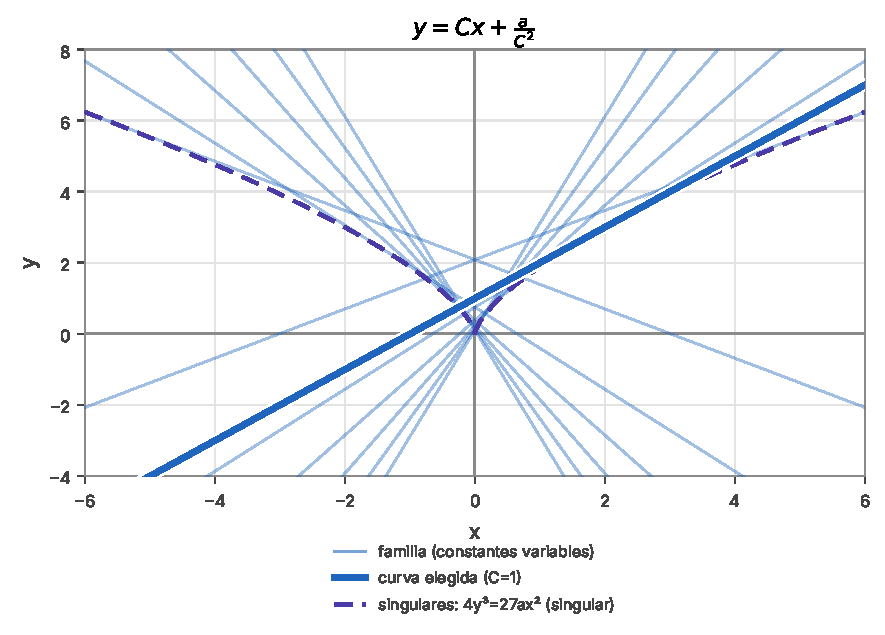
\includegraphics[width=0.8\linewidth]{h3-10.pdf}
\end{center}

\noindent\textbf{11. Integrad la EDO: $\bm{x(y')^2 - yy' - y' + 1 = 0}$} \\
Hacemos $y' = p$:
\begin{align*}
xp^2 - yp - p + 1 = 0 \implies y = xp - 1 + \frac{1}{p}
\end{align*}
\textit{$dy = pdx + xdp - \frac{1}{p^2}dp \implies \left(x - \frac{1}{p^2}\right)dp = 0$.}
\begin{itemize}
\item $dp = 0 \implies p = C \implies$ Solución general:
\[
\boxed{y = Cx + \frac{1}{C} - 1}
\]
\item $x - \dfrac{1}{p^2} = 0 \implies p = \dfrac{1}{\sqrt{x}} \implies y = 2\sqrt{x} - 1 \implies$ Solución particular:
\[
\boxed{(y+1)^2 = 4x}
\]
\end{itemize}



\begin{center}
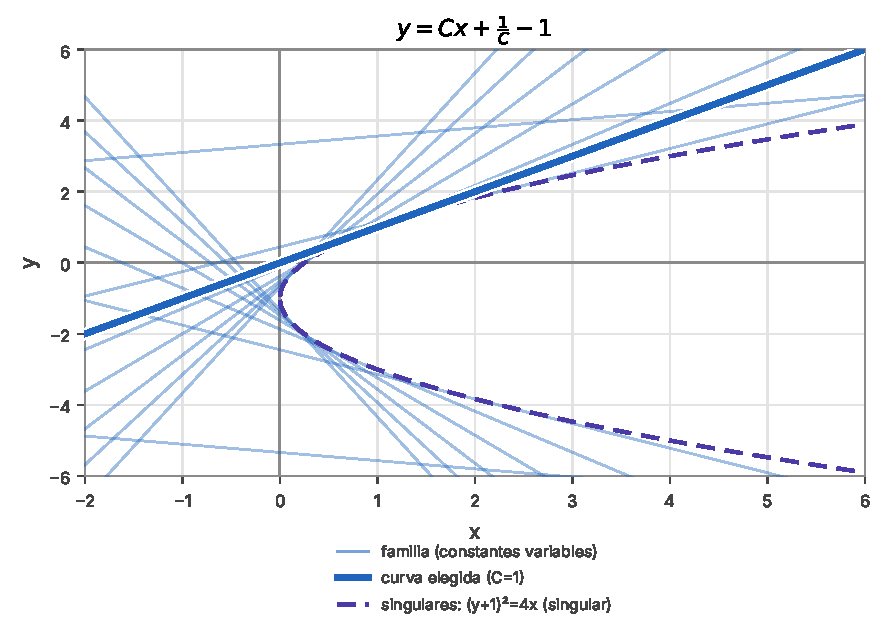
\includegraphics[width=0.8\linewidth]{h3-11.pdf}
\end{center}

\noindent\textbf{12. Integrad la EDO de Riccati: $\bm{y'e^{-x} + y^2 - 2ye^x = 1 - e^{2x}}$ sabiendo la solución $\bm{y_1 = e^x}$} \\
$y = y_1 + z = e^x + z \implies y' = e^x + z'$. Sustituyendo:
\begin{align*}
(e^x + z')e^{-x} + (e^x+z)^2 - 2(e^x+z)e^x &= 1 - e^{2x} \\
1 + z'e^{-x} + e^{2x} + 2ze^x + z^2 - 2e^{2x} - 2ze^x &= 1 - e^{2x} \implies z'e^{-x} + z^2 = 0
\end{align*}
\begin{align*}
\frac{dz}{z^2} &= -e^x dx \implies -\frac{1}{z} = -e^x - C \implies z = \frac{1}{e^x + C}
\end{align*}
\[
\boxed{y(x) = e^x + \frac{1}{e^x + C}}
\]



\begin{center}
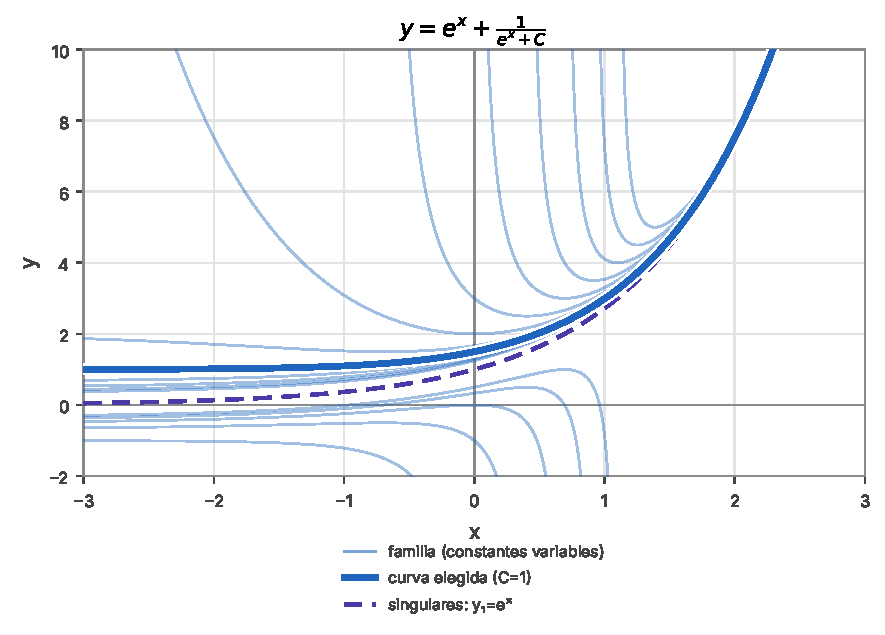
\includegraphics[width=0.8\linewidth]{h3-12.pdf}
\end{center}

\noindent\textbf{13. Hallad la solución general de la EDO de Riccati cuando $\bm{a(x):b(x):c(x) = m:n:p}$} \\
Como los coeficientes son proporcionales a constantes $m,n,p$, podemos usar $\phi(x)$ tal que $a(x) = m\phi(x)$, $b(x) = n\phi(x)$ y $c(x) = p\phi(x)$. La EDO es de variables separables:
\begin{align*}
y' + \phi(x)\big(my^2 + ny + p\big) = 0 \implies \frac{dy}{my^2 + ny + p} = -\phi(x)dx
\end{align*}
Definimos el discriminante $\Delta = n^2 - 4mp$:
\begin{itemize}
\item \textbf{ $\bm{\Delta > 0}$:} Existen dos raíces reales distintas $r_1, r_2 = \frac{-n \pm \sqrt{\Delta}}{2m}$. \\
\begin{align*}
\frac{1}{m(y-r_1)(y-r_2)} &= \frac{A}{y-r_1} + \frac{B}{y-r_2} \implies 1 = m\big[A(y-r_2) + B(y-r_1)\big]
\end{align*}
\begin{align*}
A &= \frac{1}{m(r_1 - r_2)} = \frac{1}{\sqrt{\Delta}}, \qquad B = \frac{1}{m(r_2 - r_1)} = -\frac{1}{\sqrt{\Delta}}
\end{align*}
\begin{align*}
\int \left( \frac{1/\sqrt{\Delta}}{y-r_1} - \frac{1/\sqrt{\Delta}}{y-r_2} \right) dy &= -\int \phi(x)dx \\
\frac{1}{\sqrt{\Delta}}\left(\ln|y-r_1| - \ln|y-r_2|\right) &= -\int \phi(x)dx + C_1 \implies \frac{1}{\sqrt{\Delta}}\ln\left|\frac{y-r_1}{y-r_2}\right| = -\int \phi(x)dx + C_1
\end{align*}
\[
\boxed{\frac{y-r_1}{y-r_2} = K e^{-\sqrt{\Delta}\int \phi(x)dx}}
\]

\item \textbf{$\bm{\Delta = 0}$:} raíz real doble $r = -\frac{n}{2m}$.
\begin{align*}
\int \frac{dy}{m(y + \frac{n}{2m})^2} &= -\int \phi(x)dx \implies -\frac{2}{2my+n} = -\int \phi(x)dx - C
\end{align*}
\[
\boxed{\frac{2}{2my+n} = \int \phi(x)dx + C}
\]

\item \textbf{Caso $\bm{\Delta < 0}$:} No existen raíces reales. Completando el cuadrado en el denominador:
\begin{align*}
my^2 + ny + p = m\left[\left(y + \frac{n}{2m}\right)^2 + \frac{4mp-n^2}{4m^2}\right] = m\left[\left(y + \frac{n}{2m}\right)^2 + \frac{-\Delta}{4m^2}\right]
\end{align*}
Metiendo la integral en calculadora de integrales:
\begin{align*}
\int \frac{dy}{m\left[\left(y + \frac{n}{2m}\right)^2 + \left(\frac{\sqrt{-\Delta}}{2m}\right)^2\right]} &= -\int \phi(x)dx \\
\frac{2}{\sqrt{-\Delta}}\arctan\left(\frac{2my+n}{\sqrt{-\Delta}}\right) &= -\int \phi(x)dx + C_1
\end{align*}
\[
\boxed{\arctan\left(\frac{2my+n}{\sqrt{-\Delta}}\right) = \frac{\sqrt{-\Delta}}{2}\left(C - \int \phi(x)dx\right)}
\]
\end{itemize}


\begin{center}
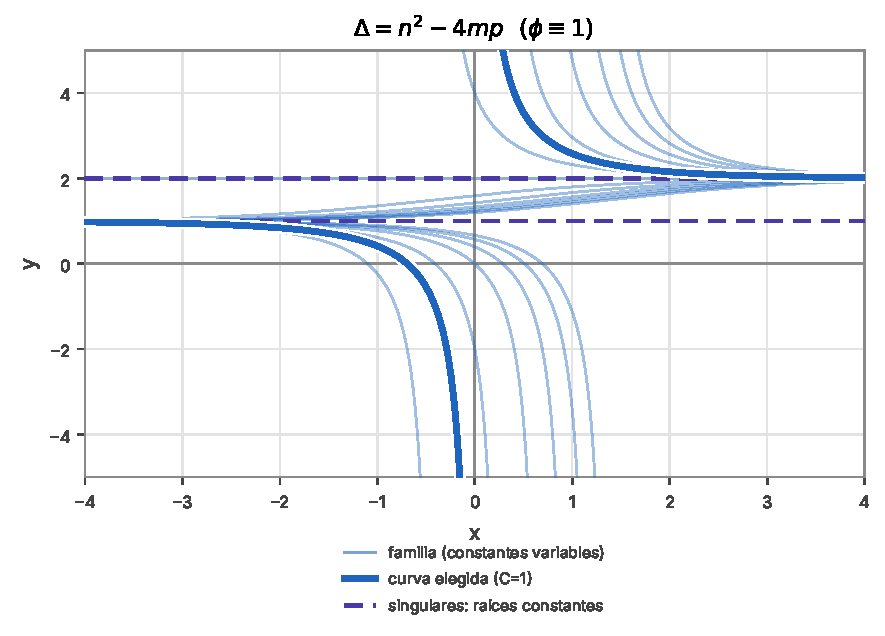
\includegraphics[width=0.8\linewidth]{h3-13.pdf}
\end{center}

\noindent\textbf{14. Construid la EDO de la familia de curvas: $\bm{y^2 = 2Cx + C^2}$} \\
\begin{align*}
2yy' = 2C \implies C = yy'
\end{align*}
\begin{align*}
y^2 = 2x(yy') + (yy')^2 \implies y^2 = 2xyy' + y^2(y')^2
\end{align*}
Dividiendo entre $y$ ($y \neq 0$):
\[
\boxed{y(y')^2 + 2xy' - y = 0}
\]



\begin{center}
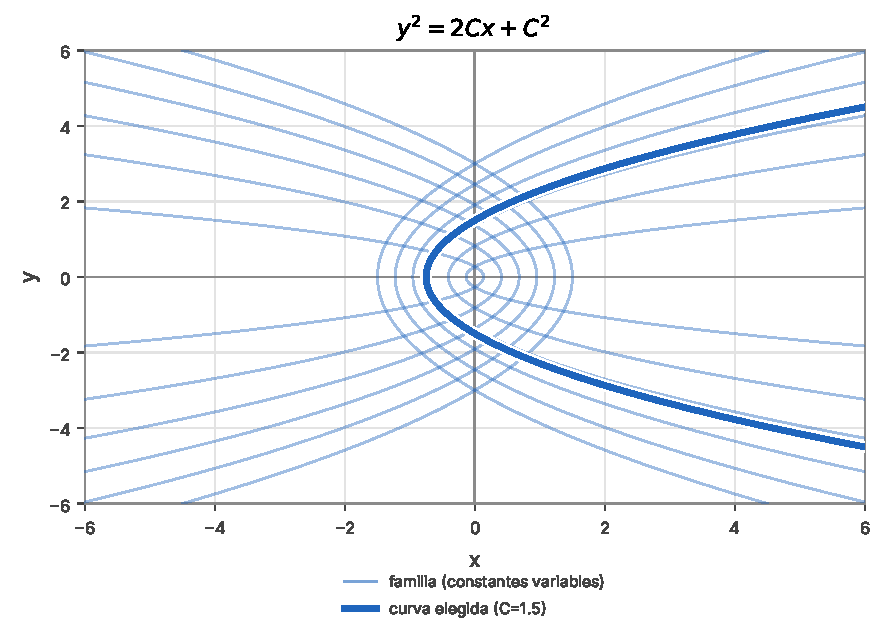
\includegraphics[width=0.8\linewidth]{h3-14.pdf}
\end{center}

\noindent\textbf{15. Construid la EDO de la familia de curvas: $\bm{y = ax^2 + bx + c}$} \\
Como la familia tiene 3 parámetros constantes ($a, b, c$), derivamos 3 veces:
\begin{align*}
y' &= 2ax + b \\
y'' &= 2a \\
y''' &= 0
\end{align*}
\[
\boxed{y''' = 0}
\]



\begin{center}
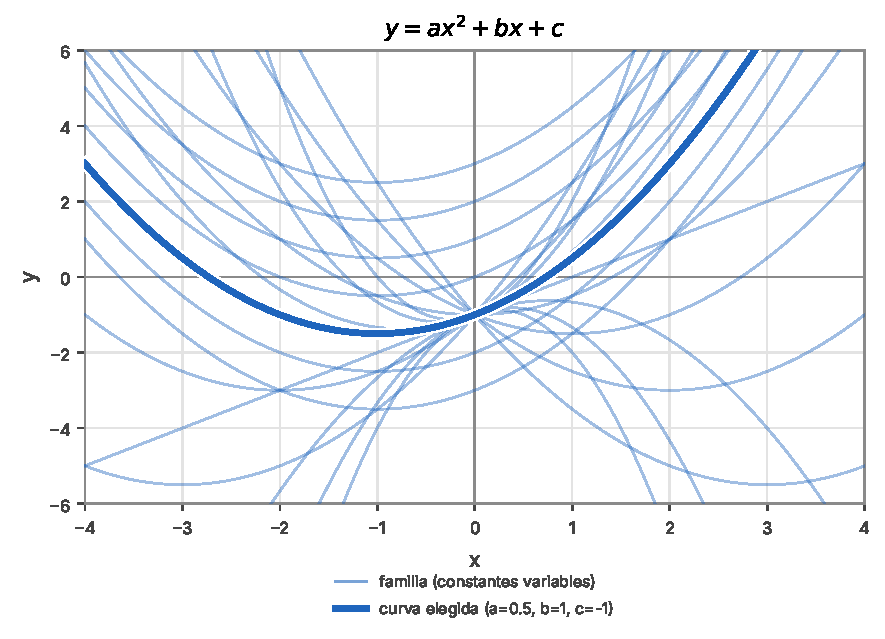
\includegraphics[width=0.8\linewidth]{h3-15.pdf}
\end{center}

\noindent\textbf{16. Construid la EDO de la familia de curvas: $\bm{y = C_1 x + C_2/x + C_3}$} \\
Como vimos en clase:
\begin{align*}
y' &= C_1 - \frac{C_2}{x^2} \\
y'' &= \frac{2C_2}{x^3} \implies C_2 = \frac{x^3 y''}{2} \\
y''' &= -\frac{6C_2}{x^4}
\end{align*}
\begin{align*}
y''' = -\frac{6}{x^4}\left(\frac{x^3 y''}{2}\right) = -\frac{3y''}{x} \implies xy''' + 3y'' = 0
\end{align*}
\[
\boxed{xy''' + 3y'' = 0}
\]



\begin{center}
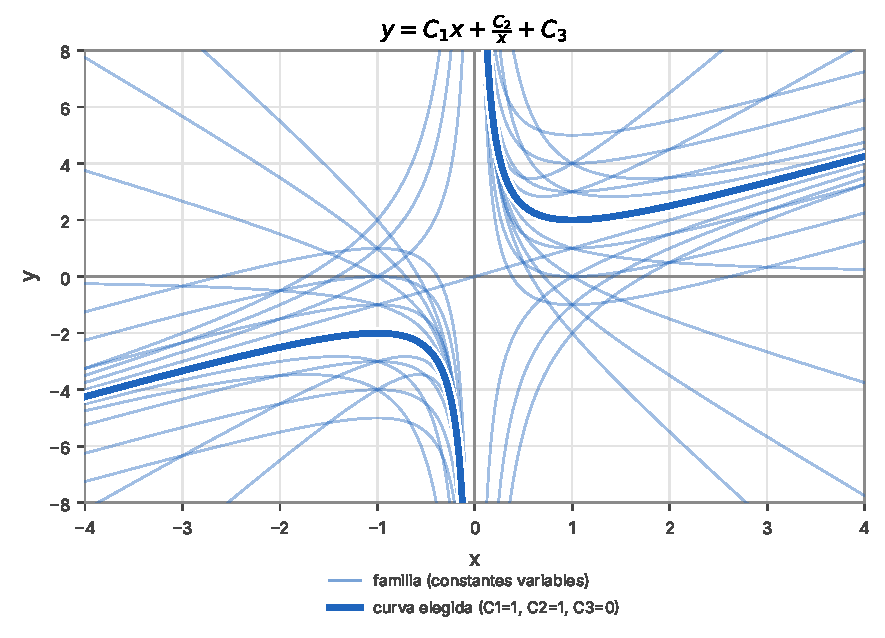
\includegraphics[width=0.8\linewidth]{h3-16.pdf}
\end{center}

\noindent\textbf{17. Hallad las trayectorias ortogonales a la familia de curvas: $\bm{y^2 + 2ax = 0}$ con $\bm{a>0}$} \\
Despejamos $a = -\frac{y^2}{2x}$ y derivamos la familia $2yy' + 2a = 0 \implies a = -yy'$.
Igualando ambas expresiones de $a$ obtenemos la EDO de la familia original:
\begin{align*}
-yy' = -\frac{y^2}{2x} \implies y' = \frac{y}{2x}
\end{align*}
$y \to \tilde{y}$ y $y' \to -\frac{1}{\tilde{y}'}$:
\begin{align*}
-\frac{1}{\tilde{y}'} = \frac{\tilde{y}}{2x} \implies \tilde{y}' = -\frac{2x}{\tilde{y}} \implies \tilde{y} \, d\tilde{y} = -2x \, dx
\end{align*}
$\frac{\tilde{y}^2}{2} = -x^2 + C_1 \implies 2x^2 + \tilde{y}^2 = C$.
\[
\boxed{2x^2 + \tilde{y}^2 = C, \qquad C > 0}
\]



\begin{center}
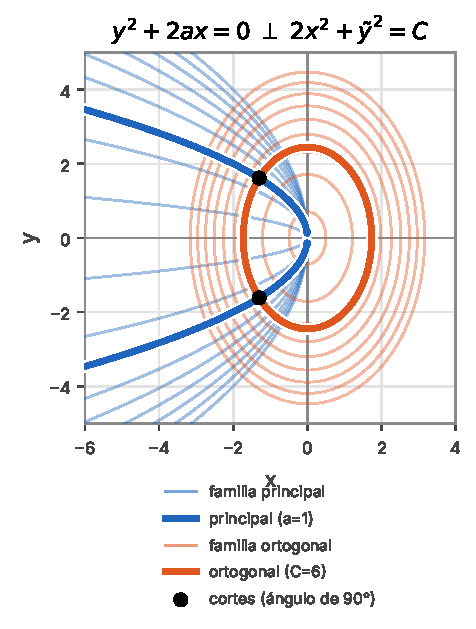
\includegraphics[width=0.8\linewidth]{h3-17.pdf}
\end{center}

\noindent\textbf{18. Hallad las trayectorias ortogonales a la familia de curvas: $\bm{y = ax^n}$ con $\bm{n}$ fijo} \\
Despejamos $a = \frac{y}{x^n}$ y derivamos $y' = nax^{n-1} = n\left(\frac{y}{x^n}\right)x^{n-1} = \frac{ny}{x}$. \\
EDO de la familia original: $y' = \frac{ny}{x}$. \\
$y \to \tilde{y}$ y $y' \to -\frac{1}{\tilde{y}'}$:
\begin{align*}
-\frac{1}{\tilde{y}'} = \frac{n\tilde{y}}{x} \implies \tilde{y}' = -\frac{x}{n\tilde{y}} \implies n\tilde{y} \, d\tilde{y} = -x \, dx
\end{align*}
$\frac{n\tilde{y}^2}{2} = -\frac{x^2}{2} + C_1$.
\[
\boxed{x^2 + n\tilde{y}^2 = C}
\]



\begin{center}
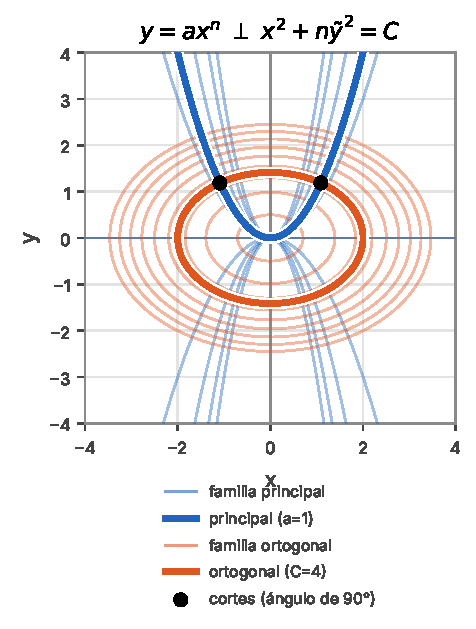
\includegraphics[width=0.8\linewidth]{h3-18.pdf}
\end{center}

\noindent\textbf{19. Hallad las trayectorias ortogonales a la familia de curvas: $\bm{y = ae^{kx}}$ con $\bm{k}$ fijo} \\
$y' = kae^{kx} = ky$. La EDO de la familia es $y' = ky$. \\
$y \to \tilde{y}$ y $y' \to -\frac{1}{\tilde{y}'}$:
\begin{align*}
-\frac{1}{\tilde{y}'} = k\tilde{y} \implies \tilde{y}' = -\frac{1}{k\tilde{y}} \implies k\tilde{y} \, d\tilde{y} = -dx
\end{align*}
$\frac{k\tilde{y}^2}{2} = -x + C_1 \implies k\tilde{y}^2 + 2x = C$.
\[
\boxed{k\tilde{y}^2 + 2x = C}
\]



\begin{center}
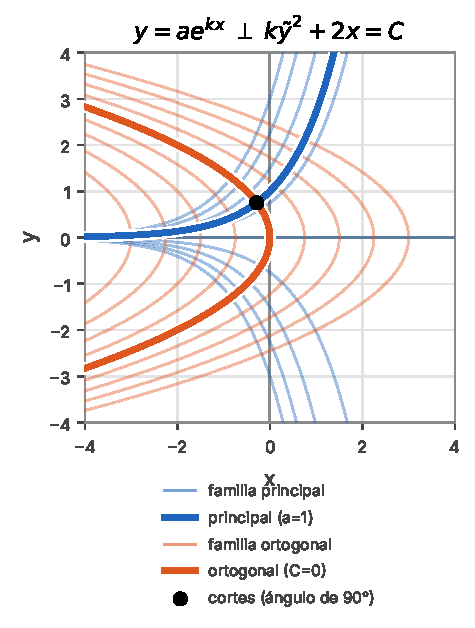
\includegraphics[width=0.8\linewidth]{h3-19.pdf}
\end{center}

\noindent\textbf{20. Hallad las trayectorias ortogonales a la familia de curvas: $\bm{\cos y = ae^{-x}}$} \\
$-\sin y \cdot y' = -ae^{-x} = -\cos y \implies y' = \cot y$. \\
$y \to \tilde{y}$ y $y' \to -\frac{1}{\tilde{y}'}$:
\begin{align*}
-\frac{1}{\tilde{y}'} = \cot \tilde{y} \implies \tilde{y}' = -\tan \tilde{y} \implies \frac{d\tilde{y}}{\tan \tilde{y}} = -dx \implies \cot \tilde{y} \, d\tilde{y} = -dx
\end{align*}
Integrando: $\ln|\sin \tilde{y}| = -x + C_1 \implies |\sin \tilde{y}| = e^{-x+C_1} = C e^{-x}$.
\[
\boxed{\sin \tilde{y} = C e^{-x}}
\]

\begin{center}
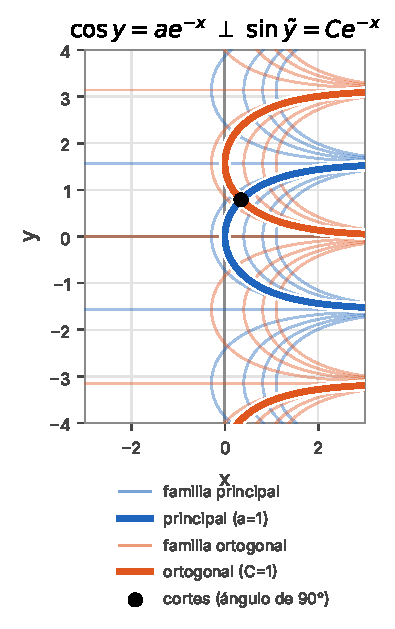
\includegraphics[width=0.8\linewidth]{h3-20.pdf}
\end{center}

\end{document}
